\hsection{Example: Packing, Cutting Stock, and Knapsack}%
%
Let's say that your family is moving to a new home in another city.
This means that you need to transport all of your belongings from your old to your new place, your PC, your clothes, maybe some furniture, a washing machine, and a refrigerator, as sketched in \cref{fig:packing_sketch}.
You cannot pack everything into your car at once, so you will have to drive back and forth a couple of times.
But how often will you have to drive?
Packing problems~\cite{S2018ITCAPOPMASM,DF1992CAPIPADATAB} aim to package sets of objects into containers as efficient as possible, i.e., in such a way that we need as few containers as possible.
Your car can be thought of as a container and whenever it is filled, you drive to the new flat.
If you need to fill the container four times, then you have to drive back and forth four times.%
%
\begin{figure}%
\centering%
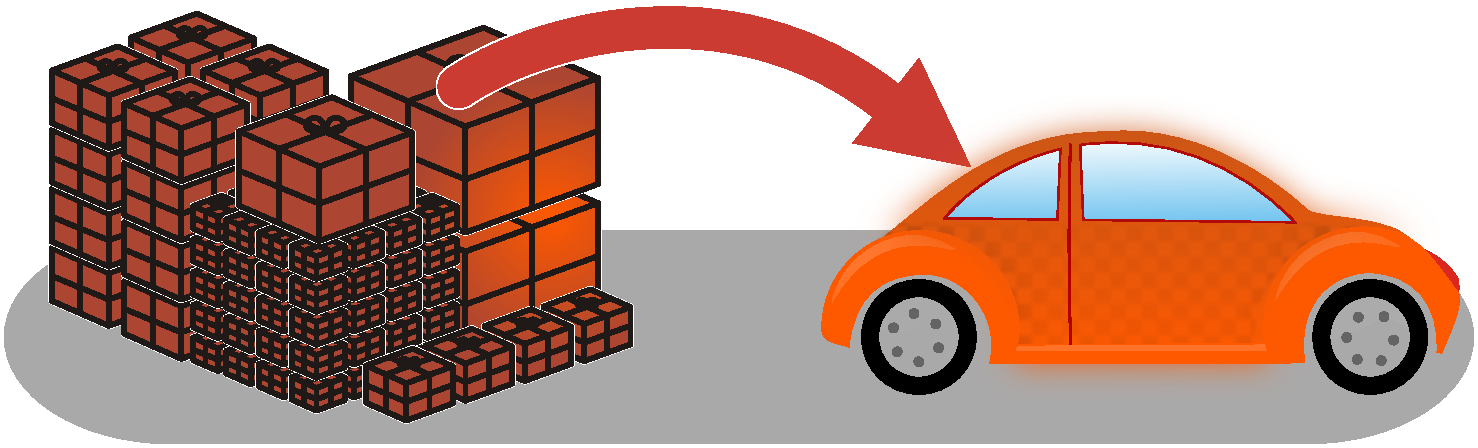
\includegraphics[width=0.8\linewidth]{\currentDir/packing_sketch}%
\caption{A sketch illustrating a packing problem.}%
\label{fig:packing_sketch}%
\end{figure}

Such \acrfullpl{BPP} exist in many variants and are very related to cutting stock problems~\cite{DF1992CAPIPADATAB}.
They can be one-dimensional~\cite{DIM2016BPACSPMMAEA}, for example if we want to transport dense/heavy objects with a truck where the maximum load weight is limiting factor while there is enough space capacity.
This is similar to having a company which puts network cables into people's homes and therefore bulk purchases reels with 100m of cables each.
Of course, each home needs a different required total length of cables and we want to cut our cables such that we need as few reels as possible.
TODO
A two-dimensional variant~\cite{LMM2002TDPPAS} could correspond to printing a set of (rectangular) images of different sizes on (rectangular) paper.
Assume that more than one image fits on a sheet of paper but we have too many images for one piece of paper.
We can cut the paper after printing to separate the single images.
We then would like to arrange the images such that we need as few sheets of paper as possible.

The three-dimensional variant then corresponds to our moving homes scenario.
Of course, there are many more different variants --- the objects we want to pack could be circular, rectangular, or have an arbitrary shape.
We may also have a limited number of containers and thus may not be able to pack all objects, in which case we would like to only package those that give us the most profit (arriving at a task called knapsack problem~\cite{MT1990KPAACI}).%
%
\endhsection%
%
